\documentclass[a4paper,12pt]{book}
\usepackage[utf8]{inputenc}

\usepackage{rachwidgets}


\newcommand{\laClass}       {CS 211}
\newcommand{\laSemester}    {Spring 2018}
\newcommand{\laChapter}     {7.2}
\newcommand{\laType}        {Exercise}
\newcommand{\laPoints}      {5}
\newcommand{\laTitle}       {Proofs about Graphs and Trees}
\newcommand{\laDate}        {}
\setcounter{chapter}{7}
\setcounter{section}{2}
\addtocounter{section}{-1}
\newcounter{question}

\toggletrue{answerkey}


\title{}
\author{Rachel Singh}
\date{\today}

\pagestyle{fancy}
\fancyhf{}

\lhead{\laClass, \laSemester, \laDate}

\chead{}

\rhead{\laChapter\ \laType\ \iftoggle{answerkey}{ KEY }{}}

\rfoot{\thepage\ of \pageref{LastPage}}

\lfoot{\scriptsize By Rachel Singh, last updated \today}

\renewcommand{\headrulewidth}{2pt}
\renewcommand{\footrulewidth}{1pt}

\begin{document}




\footnotesize
~\\ 
\textbf{\laChapter\ \laType: } In-class exercises are meant to introduce you to a new topic
and provide some practice with the new topic. Work in a team of up to 4 people to complete this exercise.
You can work simultaneously on the problems, or work separate and then check your answers with each other.
Completion score is given for this assignment.

~\\
Team:\\
(1) \tab[6cm] (2) \\
(3) \tab[6cm] (4)

\hrulefill
\normalsize 



% KEY ------------------------------------ %

\begin{enumerate}
    
    \item   
        \begin{itemize}
            \item[a.]   How many vertices does each graph have? ~\\~\\
            \begin{tabular}{p{3cm} p{3cm} p{3cm} p{3cm}}
                $G_{1}$     \solution{ 6 }{ \fitb }
                & $G_{2}$   \solution{ 6 }{ \fitb }
                & $G_{3}$   \solution{ 6 }{ \fitb }
                & $G_{4}$   \solution{ 6 }{ \fitb }
            \end{tabular}

            \item[b.]   How many edges does each graph have? ~\\~\\
            \begin{tabular}{p{3cm} p{3cm} p{3cm} p{3cm}}
                $G_{1}$     \solution{ 5 }{ \fitb }
                & $G_{2}$   \solution{ 5 }{ \fitb }
                & $G_{3}$   \solution{ 6 }{ \fitb }
                & $G_{4}$   \solution{ 4 }{ \fitb }
            \end{tabular} \vspace{0.2cm}
            \item[c.] Which graph is NOT a connected graph?
                \solution{ $G_{4}$ }{}
            \item[d.] Which of the graphs has at least one cycle?
                \solution{ $G_{3}$ }{}
            \item[e.] Which of the graphs is a tree? \solution{ $G_{1}$ and $G_{2}$. }{}
        \end{itemize}
        
    \item   
        \begin{itemize}
            \item[a.]   What is the degree of each of the vertices in $G_{1}$?
            ~\\
            \begin{tabular}{p{4cm} p{4cm} p{4cm}}
                $deg(a)$    \solution{ 1 }{ \fitb }
                & $deg(b)$  \solution{ 2 }{ \fitb }
                & $deg(c)$  \solution{ 4 }{ \fitb }
                \\
                $deg(d)$    \solution{ 1 }{ \fitb }
                & $deg(e)$  \solution{ 1 }{ \fitb }
                & $deg(f)$  \solution{ 1 }{ \fitb }
            \end{tabular}

            \item[b.]   List the leaves for $G_{1}$. \solution{ a, d, e, f }{}
        \end{itemize}
        
    \item   
        \begin{itemize}
            \item[a.]   How many edges are in your new tree?
                \solution{ 5 }{ \vspace{1cm} }
                
            \item[b.]   How many leaves on your new tree?
                \solution{ 3 }{ \vspace{1cm} }
                
            \item[c.]   If you removed one edge, would the graph still be connected?
                \solution{ no }{ \vspace{1cm} }
        \end{itemize}
        
    \item   
        \begin{itemize}
            \item[a.]  
                Is this a \textbf{subgraph}?                        \solution{ Yes }{ \vspace{0.5cm} } \\
                Are all the vertices of $G_{1}$ also nodes of $G$?  \solution{ Yes }{ \vspace{0.5cm} }  \\
                Are all the edges of $G_{1}$ also edges of $G$?     \solution{ Yes }{ \vspace{0.5cm} }
                
                
            \item[b.]   
                Is this a \textbf{subgraph}?                        \solution{ No }{ \vspace{0.5cm} } \\
                Are all the vertices of $G_{2}$ also nodes of $G$?  \solution{ Yes }{ \vspace{0.5cm} }  \\
                Are all the edges of $G_{2}$ also edges of $G$?     \solution{ No }{ \vspace{0.5cm} }
        \end{itemize}
        
        
    \item    \solution{Multiple solutions}{}

    \newpage
        
    \item   
        \solution{
            Multiple solutions depending on which node you start at, but for example...

            \begin{tabular}{p{3cm} p{3cm} p{3cm} p{3cm} }
                1. & 2. & 3. & 4.
                \\
                \begin{tikzpicture}
                    \filldraw(-1,1) circle (1pt) node [above] {a};
                \end{tikzpicture}
                &
                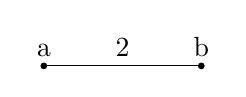
\begin{tikzpicture}
                    \filldraw(-1,1) circle (1pt) node [above] {a};
                    \filldraw(1,1) circle (1pt) node [above] {b};
                    \draw (-1,1) -- node[pos=0.5,above] {2} (1,1);
                \end{tikzpicture}
                &
                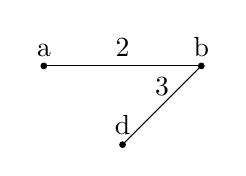
\begin{tikzpicture}
                    \filldraw(-1,1) circle (1pt) node [above] {a};
                    \filldraw(1,1) circle (1pt) node [above] {b};
                    \filldraw (0,   0)  circle (1pt)    node[above]     {d};
                    \draw (-1,1) -- node[pos=0.5,above] {2} (1,1);
                    \draw (1,1) -- node[pos=0.5,above] {3} (0,0);
                \end{tikzpicture}
                &
                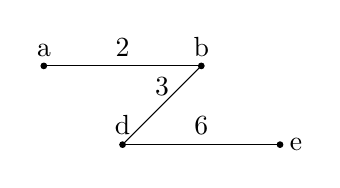
\begin{tikzpicture}
                    \filldraw(-1,1) circle (1pt) node [above] {a};
                    \filldraw(1,1) circle (1pt) node [above] {b};
                    \filldraw (0,   0)  circle (1pt)    node[above]     {d};
                    \filldraw (2,   0)  circle (1pt)    node[right]     {e};
                    \draw (-1,1) -- node[pos=0.5,above] {2} (1,1);
                    \draw (1,1) -- node[pos=0.5,above] {3} (0,0);
                    \draw (0,0) -- node[pos=0.5,above] {6} (2,0);
                \end{tikzpicture}
            \end{tabular}

            \hrulefill
            
            \begin{tabular}{p{6cm}  p{6cm} }
                5. & 6.
                \\
                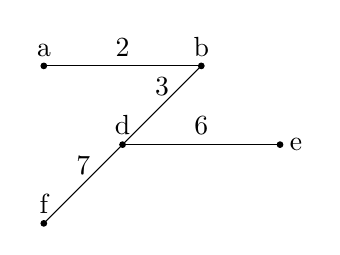
\begin{tikzpicture}
                    \filldraw(-1,1) circle (1pt) node [above] {a};
                    \filldraw(1,1) circle (1pt) node [above] {b};
                    \filldraw (0,   0)  circle (1pt)    node[above]     {d};
                    \filldraw (-1,  -1) circle (1pt)    node[above]     {f};
                    \filldraw (2,   0)  circle (1pt)    node[right]     {e};
                    \draw (-1,1) -- node[pos=0.5,above] {2} (1,1);
                    \draw (1,1) -- node[pos=0.5,above] {3} (0,0);
                    \draw (0,0) -- node[pos=0.5,above] {7} (-1,-1);
                    \draw (0,0) -- node[pos=0.5,above] {6} (2,0);
                \end{tikzpicture}
                &
                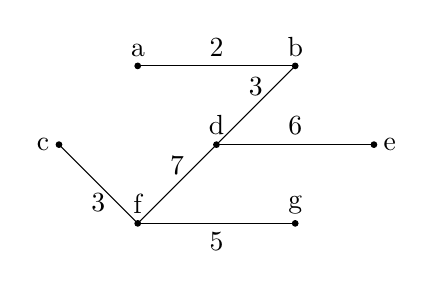
\begin{tikzpicture}
                    \filldraw(-1,1) circle (1pt) node [above] {a};
                    \filldraw(1,1) circle (1pt) node [above] {b};
                    \filldraw (0,   0)  circle (1pt)    node[above]     {d};
                    \filldraw (-1,  -1) circle (1pt)    node[above]     {f};
                    \filldraw (-2,  0)  circle (1pt)    node[left]      {c};
                    \filldraw (2,   0)  circle (1pt)    node[right]     {e};
                    \filldraw (1,   -1) circle (1pt)    node[above]     {g};
                    \draw (-1,1) -- node[pos=0.5,above] {2} (1,1);
                    \draw (1,1) -- node[pos=0.5,above] {3} (0,0);
                    \draw (0,0) -- node[pos=0.5,above] {7} (-1,-1);
                    \draw (0,0) -- node[pos=0.5,above] {6} (2,0);
                    \draw (-1,-1) -- node[pos=0.5,below] {3} (-2,0);
                    \draw (-1,-1) -- node[pos=0.5,below] {5} (1,-1);
                \end{tikzpicture}
            \end{tabular}

            \hrulefill
            
            \begin{tabular}{p{6cm}  p{6cm} }
                7. \\
                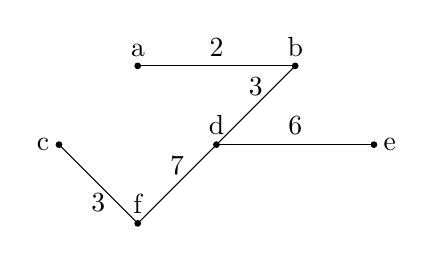
\begin{tikzpicture}
                    \filldraw(-1,1) circle (1pt) node [above] {a};
                    \filldraw(1,1) circle (1pt) node [above] {b};
                    \filldraw (0,   0)  circle (1pt)    node[above]     {d};
                    \filldraw (-1,  -1) circle (1pt)    node[above]     {f};
                    \filldraw (-2,  0)  circle (1pt)    node[left]      {c};
                    \filldraw (2,   0)  circle (1pt)    node[right]     {e};
                    \draw (-1,1) -- node[pos=0.5,above] {2} (1,1);
                    \draw (1,1) -- node[pos=0.5,above] {3} (0,0);
                    \draw (0,0) -- node[pos=0.5,above] {7} (-1,-1);
                    \draw (0,0) -- node[pos=0.5,above] {6} (2,0);
                    \draw (-1,-1) -- node[pos=0.5,below] {3} (-2,0);
                \end{tikzpicture}
            \end{tabular}
        }{}
        
\end{enumerate}




\end{document}

